\documentclass[12pt,a4paper]{article}
\usepackage{tikz}
\usepackage{graphicx}
\usepackage{hyperref}
\usepackage{verbatim}
\usepackage[font=small,labelfont=bf]{caption}
\usepackage{geometry}
%\geometry{showframe=true}
\geometry{a4paper,margin=1.25in}

\usepackage[right]{lineno}
\nolinenumbers
\linenumbers
\modulolinenumbers[5]
%\usepackage[printwatermark]{xwatermark}
\usepackage{draftwatermark}
\SetWatermarkText{DRAFT}
\SetWatermarkScale{10}
\SetWatermarkLightness{.975}
\usepackage{amsmath}
\usepackage{color}
\usepackage{caption,float}
\usepackage{icomma}
\captionsetup[table]{skip=8pt}
\newcommand{\millper}{ &\multicolumn{3}{c}{\textsc{aud millions}}
  &\multicolumn{3}{c}{\textsc{percentages}}\\}

\newcommand{\labper}{ &\multicolumn{3}{l}{\textsc{fte employees}}&
  \multicolumn{3}{r}{\textsc{percentages}}\\}

%\usepackage{_tex/preamble-files/paper-preamble}

\title{Boyne Smelters\\\vskip5pt
  \large{Economic Impact on the
  Gladstone Region and Queensland}}
\author{\small Patrick O’Callaghan and John Mangan}
\renewcommand\thefigure{(\roman{figure})}
\begin{document}

\maketitle

%\section*{\centering Draft}

\paragraph{Outline} Australia is one of only three countries in the world with
a fully integrated supply chain for producing Aluminium
\cite{GN-Aluminium-smelters}. In particular, Bauxite from Weipa, North
Queensland, is refined and smelted in Gladstone, Central Queensland.  Aluminium
smelting is a highly energy intensive process with Boyne Smelter Limited (BSL)
in Gladstone consuming approximately one eighth of the total electricity supply
of Queensland over the course of a typical year. Like other regions that
produce aluminium, Central Queensland is energy-abundant with an active
coal-mining and natural-gas industry. The smelter is supported by the
coal-fired Gladstone Power Station (GPS). 

GPS has the capacity to supply one quarter of Queenland's annual electricity
demand. GPS is unique in that it carries a variable load with the ability to
quickly increase the supply of power in the case of an extended blackout that
would otherwise lead to aluminium freezing the pipes and costly damages to BSL.

In this paper, we study the economic impact of a permanent closure of the
smelter on the Gladstone region. The key local variables of interest are
capital, output, consumption as well as gross value added and employment which
we model across sectors and over time. We model the broader gladstone region
and estimate the impact on the broader supply chain via imports and exports. We
present results for the standard 19 ANZSIC divisions and for the economy on
aggregate.


\paragraph{Summary of results} The sectors where there is an impact of
substance are Agriculture, Mining, Manufacturing and Utilities. These are
ANZSIC divisions A, B, C and D respectively. Our presentation and analysis of
results focuses on these sectors.  In brief, manufacturing and utilities are
both permanently worse off relative to the no-closure status quo.  In contrast,
mining and, to a lesser extent, agriculture are permanently better off with
investment and employment in these sectors increasing immediately after the
shock.

Relative to status quo, when labour is mobile, the positive response by mining
and agriculture reduces the immediate shock to aggregate output to just under
1.5\% and the economy has caught up within 10 years.  When labour is immobile,
the immediate shock to aggregate output is just under 6\%, and the economy
remains 1\% smaller than under the status quo in the long run. The truth is
likely to lie somewhere in between. The impact on consumption is small but
positive for the same reason that mining and agriculture respond positively:
the price of utility goods (such as electricity and water) permanently fall by
10\% as a result of the closure. In future work we will exploit the flexible
nature of our intertemporal modelling approach to explore the case where
Utilities prices remain high due to the fact that Gladstone is connected to the
National Electricity Market.

\paragraph{The Gladstone Economy} To come from \cite{glad-prospectus} and
the 2020 report for QTC.

\paragraph{Background to the shock} Prior to the closure of the smelter, we
assume that all sectors of the economy grow at a rate of 1.5\% to 1.8\% and
that their growth path is balanced. Thus the stock variable capital grows at
approximately the same rate as flow variables such as output.  This assumption
is justified by virtue of the fact that BSL is forty years old, and much of the
local aluminium industry was established in the sixties and seventies.  The
main exception is Gladstone's second alumina refinery, Yarwun Alumina Refinery
(YAR), which opened in 2004.

\paragraph{Current capital} Direct estimates of current capital per sector are
unavailable at the regional level. To do so, we exploit the intertemporal
features of our model to evolve the economy optimally and endogenously over a
long period of time (approximately 70 years).  This approach ensures that, at
the time of the shock, the distribution of capital across sectors, at the time
of the shock, is independent of the initial distribution of capital.  Indeed,
current capital depends only on the parameters of the model with our estimates
of productivity factors and investment flows playing a key role. 

\subsection*{Estimating the parameters} Our first source of data for estimating
the share parameters of the model are the 2019 ABS input-output
tables (5 and 8) for the Australian economy. Table 8 provides a full account of
the individual flows from sector to sector and from sector to household and
government.  For example, the flow of goods (such as bauxite) from the mining
sector to the manufacturing sector is a combination of local and imported goods
and an estimate of the total value of this flow can be found on table 8.  An
estimate of the domestic share of this composite flow can be found on table 5
and imports are found by taking the difference between table 8 and table 5.
For the present study, we aggregate the above tables from 114 IOIG industries
to the 19 ANSIC divisions (A, B, C, ..., S). 

The second source of data is the 1997 US “Make” and Capital/investment Flows
tables from the Bureau of Economic Analysis in the US. This is a commonly used
table that also features in the influential paper \cite{Atalay}.
We were able to adapt this to the 2019 Australian economy on the basis of
investment (Gross Fixed Capital Formation) data from the Australian
input-output tables and the GFCF by Industry by Asset type tables, also from
the ABS. With minor modifications, the traditional RAS method/algorithm works
well to ensure row column balance for this table in isolation.

We regionalise the above tables using a combination of 2016 census data and
Remplan so as to bring the economy as close as possible to the current
Gladstone economy.\footnote{We will replace this data in due course with data
from latest census and local industry data from BLADE.} Regionalising national
account data in a top-down manner is inherently imprecise and difficult. To
ensure robustness of our results, we created three different versions of the
Gladstone economy using two different methods which we now describe.
Regardless of method, the main results all point in the same direction. Our
reasons for preferring the second method are that the resulting collection of
tables not only look more reasonable, they also perform better with the
model.

The first method is the traditional RAS technique where (given estimates of
sectoral output, employment imports and exports for a region) one estimates the
individual flows between sectors by minimising the \emph{relative} entropy
subject to row-column balance (a form of regional accounting).\footnote{
  Relative to the Australian input-output tables mentioned above.  }

%This method often yielded tables that
%were clearly unusable for the model and the process of trying to fix the
%associated problems is very time consuming and still has no guarantee of
%accuracy for measuring the relative importance of different transactions.

The second method is more targeted. It involves the assumption of constant
returns to scale and, whilst keeping the Australian economy broadly intact,
using accurate data on specific flows between sectors, households and exports,
we make specific modifications to the table. In contrast with the first method,
no attempt is made to ensure the table is balanced. 
%
%We argue that this second method is more appropriate for a number of reasons:
%
%\begin{enumerate}
%    
%  \item it allows us to ensure that key transactions are well-modelled without
%  excessive distorting the rest of the table: something that is typical of the
%  RAS method;
%
%  \item we have an initial ``burn-in'' phase of 70 periods where the economy
%  evolves to account for the modifications that we have made.  In future work,
%  we will allow parameters to evolve during this phase.
%
%  \item the RAS method is intended to replicate a form of re-equilibration
%  process and this is what our burn-in phase achieves.
%
%  \item although a canonical CGE model can replicate the national accounts
%  data as an equilibrium for a given year, it cannot do so at the regional
%  level because the data is not available. 
%
%\item on a technical point, it is really only the relative importance that
%matters for estimating share parameters
%
%  \item The resulting collection of tables work extremely well with the
%  computational model.
%
%\end{enumerate}
%
Instead, we focus on ensuring that key transactions are in proportion to what
we observe in available data. In particular, we obtain precise estimates for
the cost structure of the Aluminium sector and scale up key transactions for
electricity supply in accordance with data on output from the Rio Tinto annual
accounts (\cite{RT}), electricity prices (\cite{AEMO}), export and import data
from Gladstone port (\cite{port}, and well-known estimates of cost from sources
on aluminium production such as \cite{GN-Aluminium-smelters} and \cite{bat}.
We then run the ``burn-in phase" for a variety of parameters and choose those
that yield an economy that best matches the regional data we have.  Our main
concern with the second method is the risk that the tables we have generated
paint a more diverse picture of the Gladstone economy than is in fact the case.
That is to say, there is the possibility that some other sectors are more
reliant on the smelter than our results suggest. We propose to deal with this
concern by conducting systematic robustness checks for a wider variety of
parameters.

\paragraph{The parameters in detail} A sample of the productivity parameters
that we calibrate through the burn-in phase are the following:

\begin{table}[H]
\centering
  \caption{\label{tab-prod} Productivity parameters per sector}
\begin{tabular}{l|l|l|l|l|l|l|l|l|l|l|l}

  Divisions &  A  & B  & C  & D  & E  & \dots  & I  & J  & K  & L & \dots \\

\hline

  No shock & 31.2 & 31.7 & 32.6 & 21.9 & 31.6 & \dots & 31.4 & 31.1 & 21.8 &
  21.9 & \dots\\

\hline

  Shock & 31.2 & 31.7 & {\color{red}26.1} & 21.9 & 31.6 & \dots & 31.4 & 31.1 &
  21.8 & 21.9 & \dots\\

\end{tabular}
\end{table}
 
Initially productivity parameters were simply set using standard approaches
such as formulas for the minimum unit cost. Since this did not produce
reasonable output values in the long run, we adjusted these values to reflect
the higher output in sectors where output is higher.  These modifications are
relatively small on the whole.  The only exceptions were to divisions D
(Utilities), K (Finance) and L (Real Estate). These were set at 70\% of the
levels that were assigned using standard methods such as the minimum cost of
producing a unit adjusted by regional output per sector.  The reason for this
is that otherwise these sectors become excessively large during the burn-in
phase. Division L is where the exceptional IOIG sector ``Ownership of
Dwellings" is allocated. Ownership of dwellings constitutes 30\% of all gross
fixed capital formation as per ABS data. Arguably this is relatively
unproductive capital given that it is essentially housing.


In table \ref{tab-prod} we see that the shock entails a 20\% fall in the
productivity of manufacturing (C). This, on the one hand, is necessary because
otherwise the endogenous optimal investment process will simply return capital
to its previous state as if the smelter had never closed. On the other, we
argue that such a fall in productivity is reasonable given that the Aluminium
sector is so well vertically-integrated.  It can also be viewed as capturing
perception of higher risk of investing in Gladstone manufacturing after the
closure of the smelter.

To specialise the Australian table to Gladstone, the key transactions for which
we adjust parameters are the following (all specialisation ratios are relative to
Australia):

\begin{enumerate}
  \item exports of Manufacturing are three times domestic usage.
\item the specialisation ratio for Mining purchases by manufacturing is 2.
\item the specialisation ratio for Manufacturing purchases by manufacturing is
  1.5.
\item the specialisation ratio for Utility (electricity and water) purchases by
  Manufacturing is 7.
\item the specialisation ratio for imported Mining goods (such as bauxite) is
  5.
\item finally, we include the subsidy as a payment to capital.
\end{enumerate}

According to our calculations, the subsidy to aluminium amounts to
\$174\textsc{m}.


\paragraph{Subsidies} to aluminium smelting have been well-debated in Australia
for over 20 years \cite{subsidies}. In 2015, the Government-Owned Corporation
CS Energy  described its contractual obligation to GPS as onerous \cite[page
10]{CSE}.

In our calculations, we assume that BSL pays around $\$60$ per \textsc{mwh}.
This is significantly lower than current wholesale future electricity prices of
around \$120 for the calendar year 2023 \cite{aer}. Assuming that BSL would pay wholesale
prices in the absence of a subsidy, we estimate that the subsidy per
\textsc{mwh} to aluminium production at BSL is $\$60 $.  Given that
$14\textsc{mwh}$ are required to produce a single tonne of aluminium, and BSL
currently produces $502 \textsc{kt}$ per annum, we are able to obtain an estimate of the
current subsidy to aluminium production at BSL, approximately \[\$
419.16\textsc{m} = \$60 \cdot 14 \cdot 499\textsc{k} \] 


\begin{figure}[H] \caption{  \label{fig-Bx-ratio} The structure of the
  Interconnection and Power Pooling Agreement}
  \includegraphics[width=0.95\textwidth]{./ippa.png} \vskip5pt
  \caption*{\footnotesize CSE sells GPS's Electricity output at wholesale
  prices (\$120) and sells the base load quantity of approximately
  $7,000\textsc{gwh}$ per annum back to BSL (indirectly via GPS) at prices net
  of subsidy (\$60). This has lead it to publicly describe its contract with
  GPS as onerous \cite{CSE}.} \end{figure}
\begin{figure}[H]
    \caption{\label{fig-heatAcomp} The input-output matrix (\textsc{aud}
    millions) for the status quo Gladstone economy}
  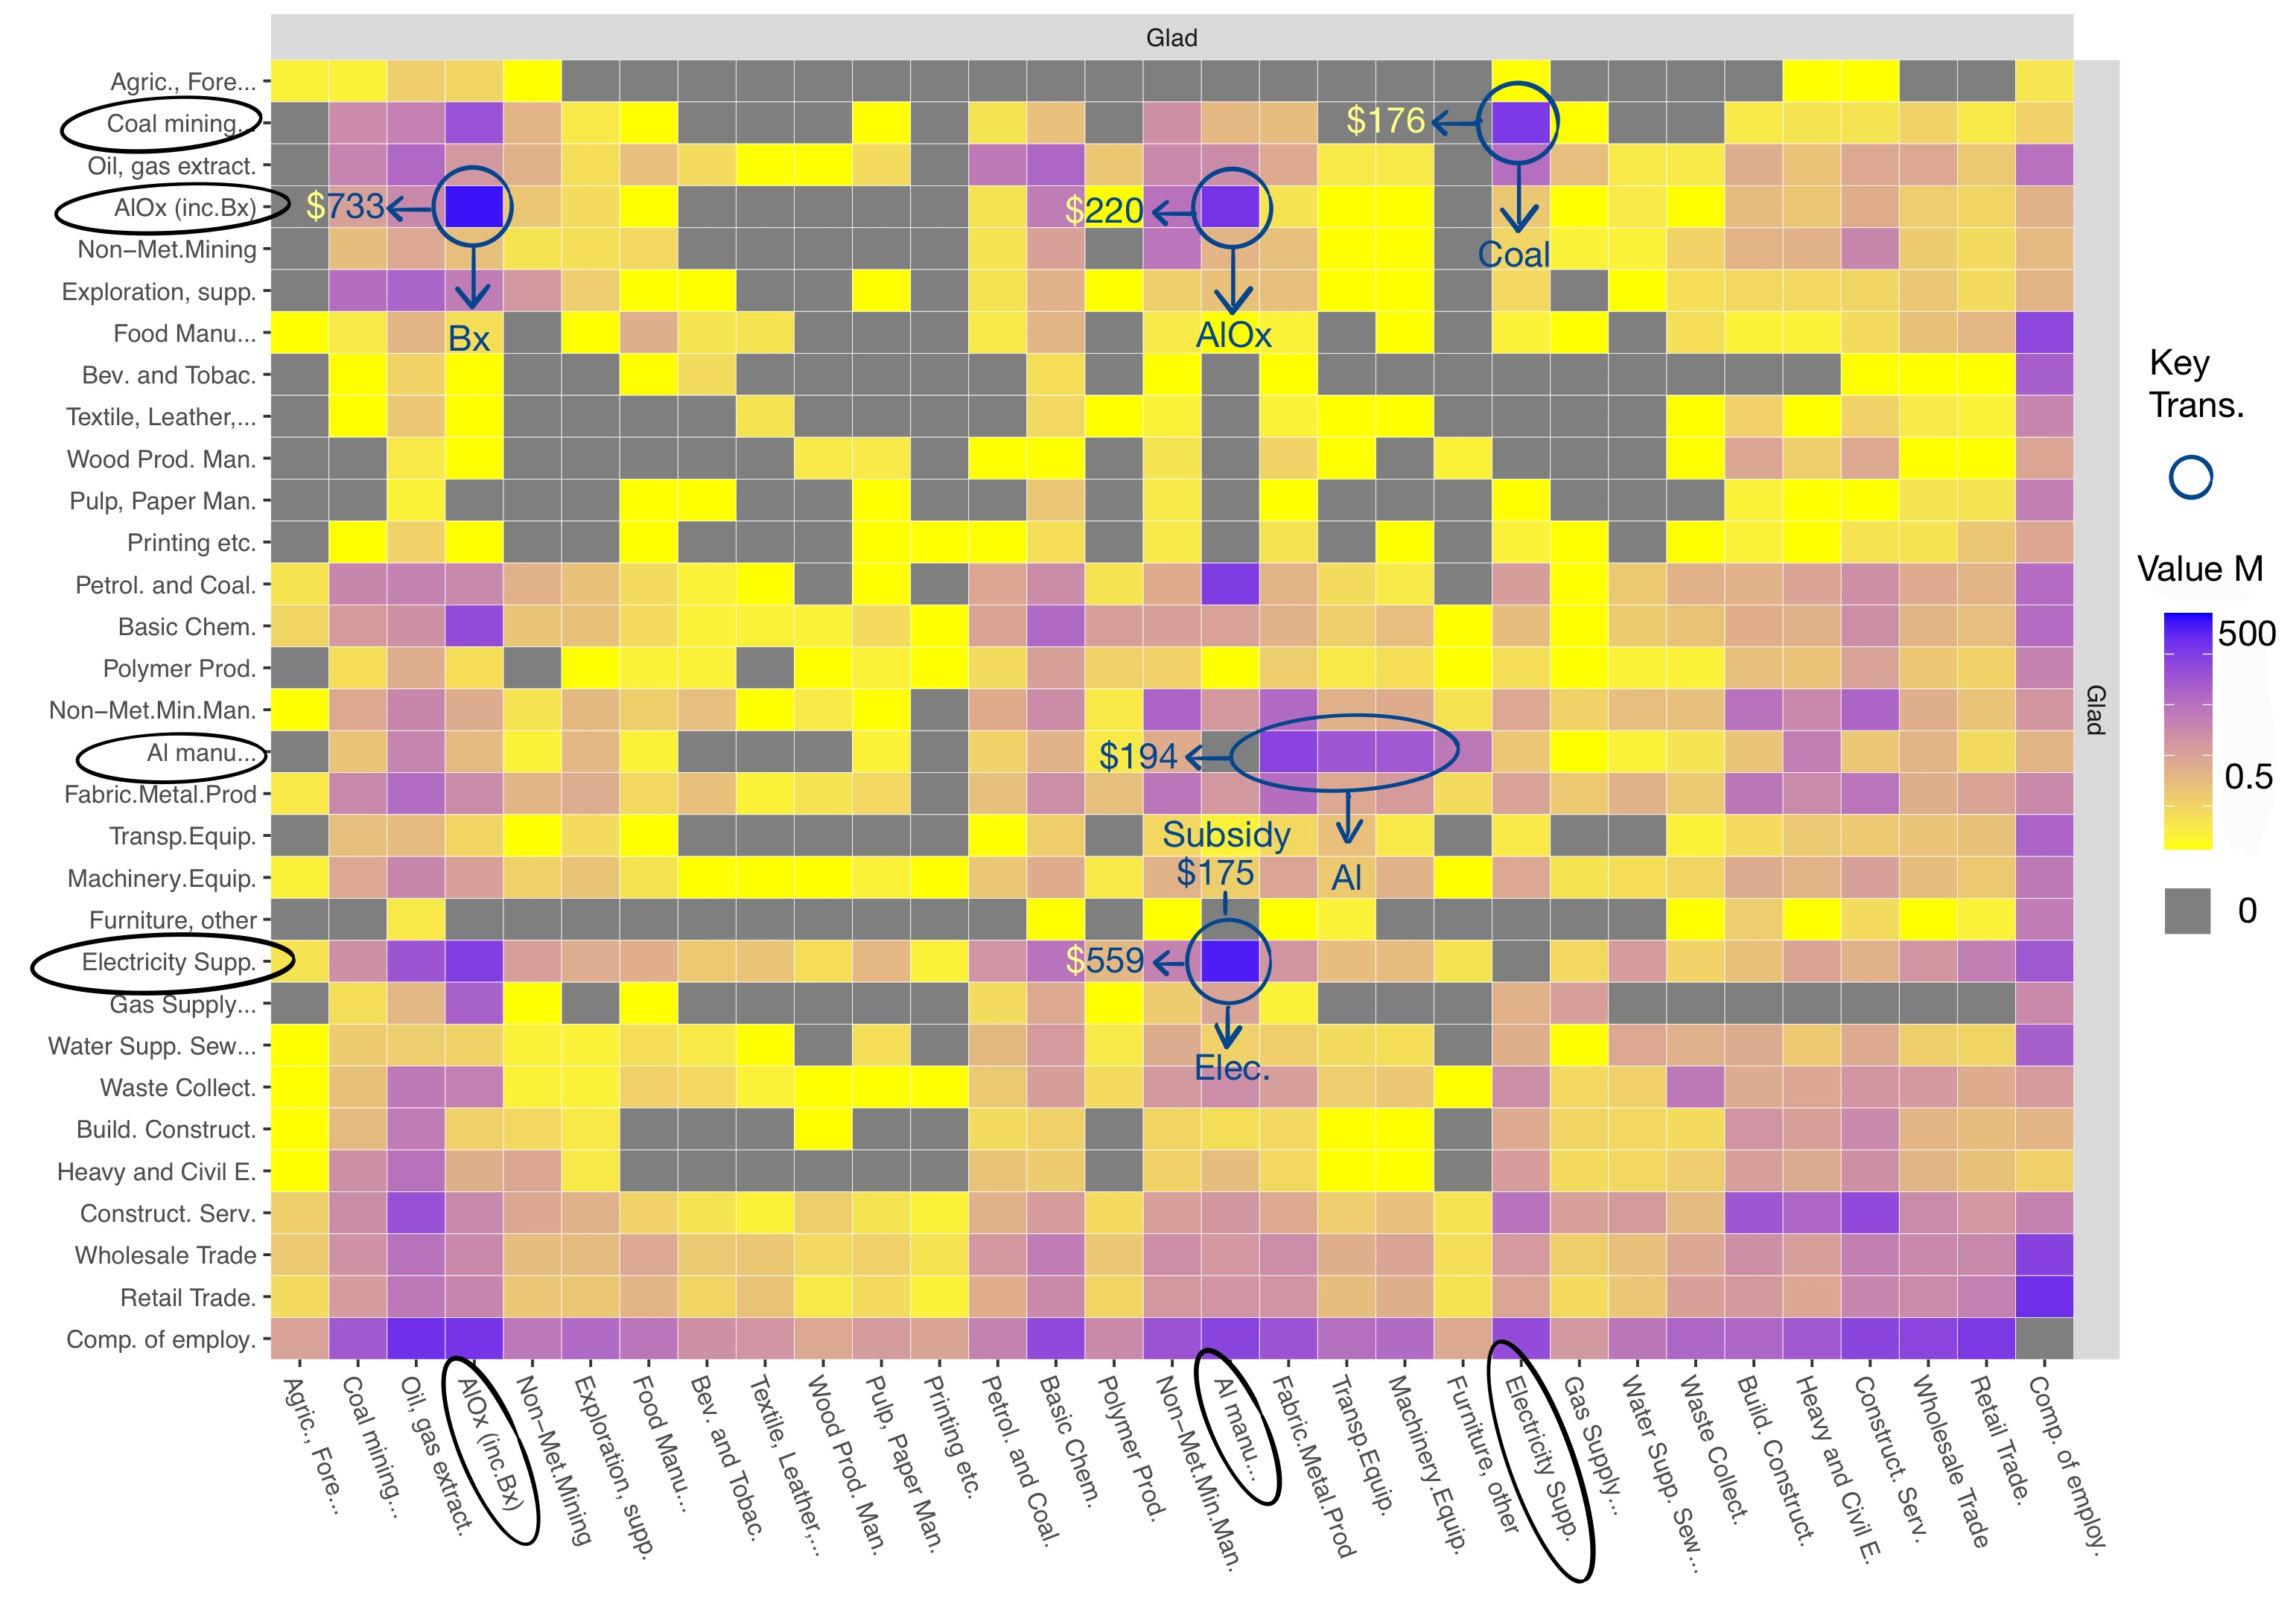
\includegraphics[width=.95\textwidth]{./heatZvalcomp-ann.jpg} \caption*{
    In this heatmap, key, large transactions are represented by blue or violet
    squares. Yellow transactions are smaller. Grey stands for zero/no
    transaction.  }
\end{figure}

\paragraph{Summary of status quo economy} The final values for flows between
sectors are intended to capture the key features of figure \ref{fig-heatAcomp}
a table that we constructed for a previous report for QTC. Figure
\ref{fig-heatAcomp} presents data of the same type as table 8: composite flows
of domestic and imported goods.  For the present study, we need to pair this
data with estimates of a richer set of parameters which we derive from table 5
and US capital flows.


\paragraph{The shock}
Aside from the
{\color{red} 20\%} shock to productivity and the {\color{red}25\%} reduction in
manufacturing capital, the scenarios involve modifying status quo transactions
as follows:
\begin{enumerate}
    
  \item exports of Manufacturing goods decrease by {\color{red}25\%}
    
  \item purchases of Mining goods by Manufacturing decrease by {\color{red}
    10\%}

  \item purchases of Manufacturing goods by the Manufacturing sector decrease
    by {\color{red} 60\%}. This may seem high, but it is in line with the fact
    that, in Gladstone, most goods are manufactured for export.

  \item purchases of Utility goods by the Manufacturing sector decrease by
    {\color{red}85\%}. This significant part of the shock is in line with the
    fact that the smelter consumes one eighth of Queensland's electricity
    output.
    
\end{enumerate}

\subsection*{More detailed analysis of results}

\paragraph{Overview} Under the assumption that the Gladstone economy remains on
a balanced growth path of 1.5\% to 1.8\% across all sectors, the main takeaway
is that only Manufacturing and Utilities are significantly affected in a
negative way. In fact, Mining and Agriculture benefit from the lower prices for
Utilities and Manufacturing goods as well as an improvement in their relative
productivity (relative to Manufacturing). On aggregate, although output, Gross
Value Added, employment and exports all fall, consumption is weakly, yet
positively (between 0\% and 1\%) improved as a result of lower prices.

In practice, the 10\% fall in Utilities price may be tempered by the fact that
Gladstone is connected to the National Electricity Market and so the benefit of
lower demand for electricity from the smelter would be spread over a much
larger region and population. Indeed for the same reason, the impact on prices
is likely to be smaller. This will temper the gains to aggregate consumption.
The same holds for the gains to the Mining and Agricultural sectors.

\begin{figure}[H]
  \caption{Aggregate: percentage change relative to status quo
 over time in years
  \label{fig-agg-change}}
 
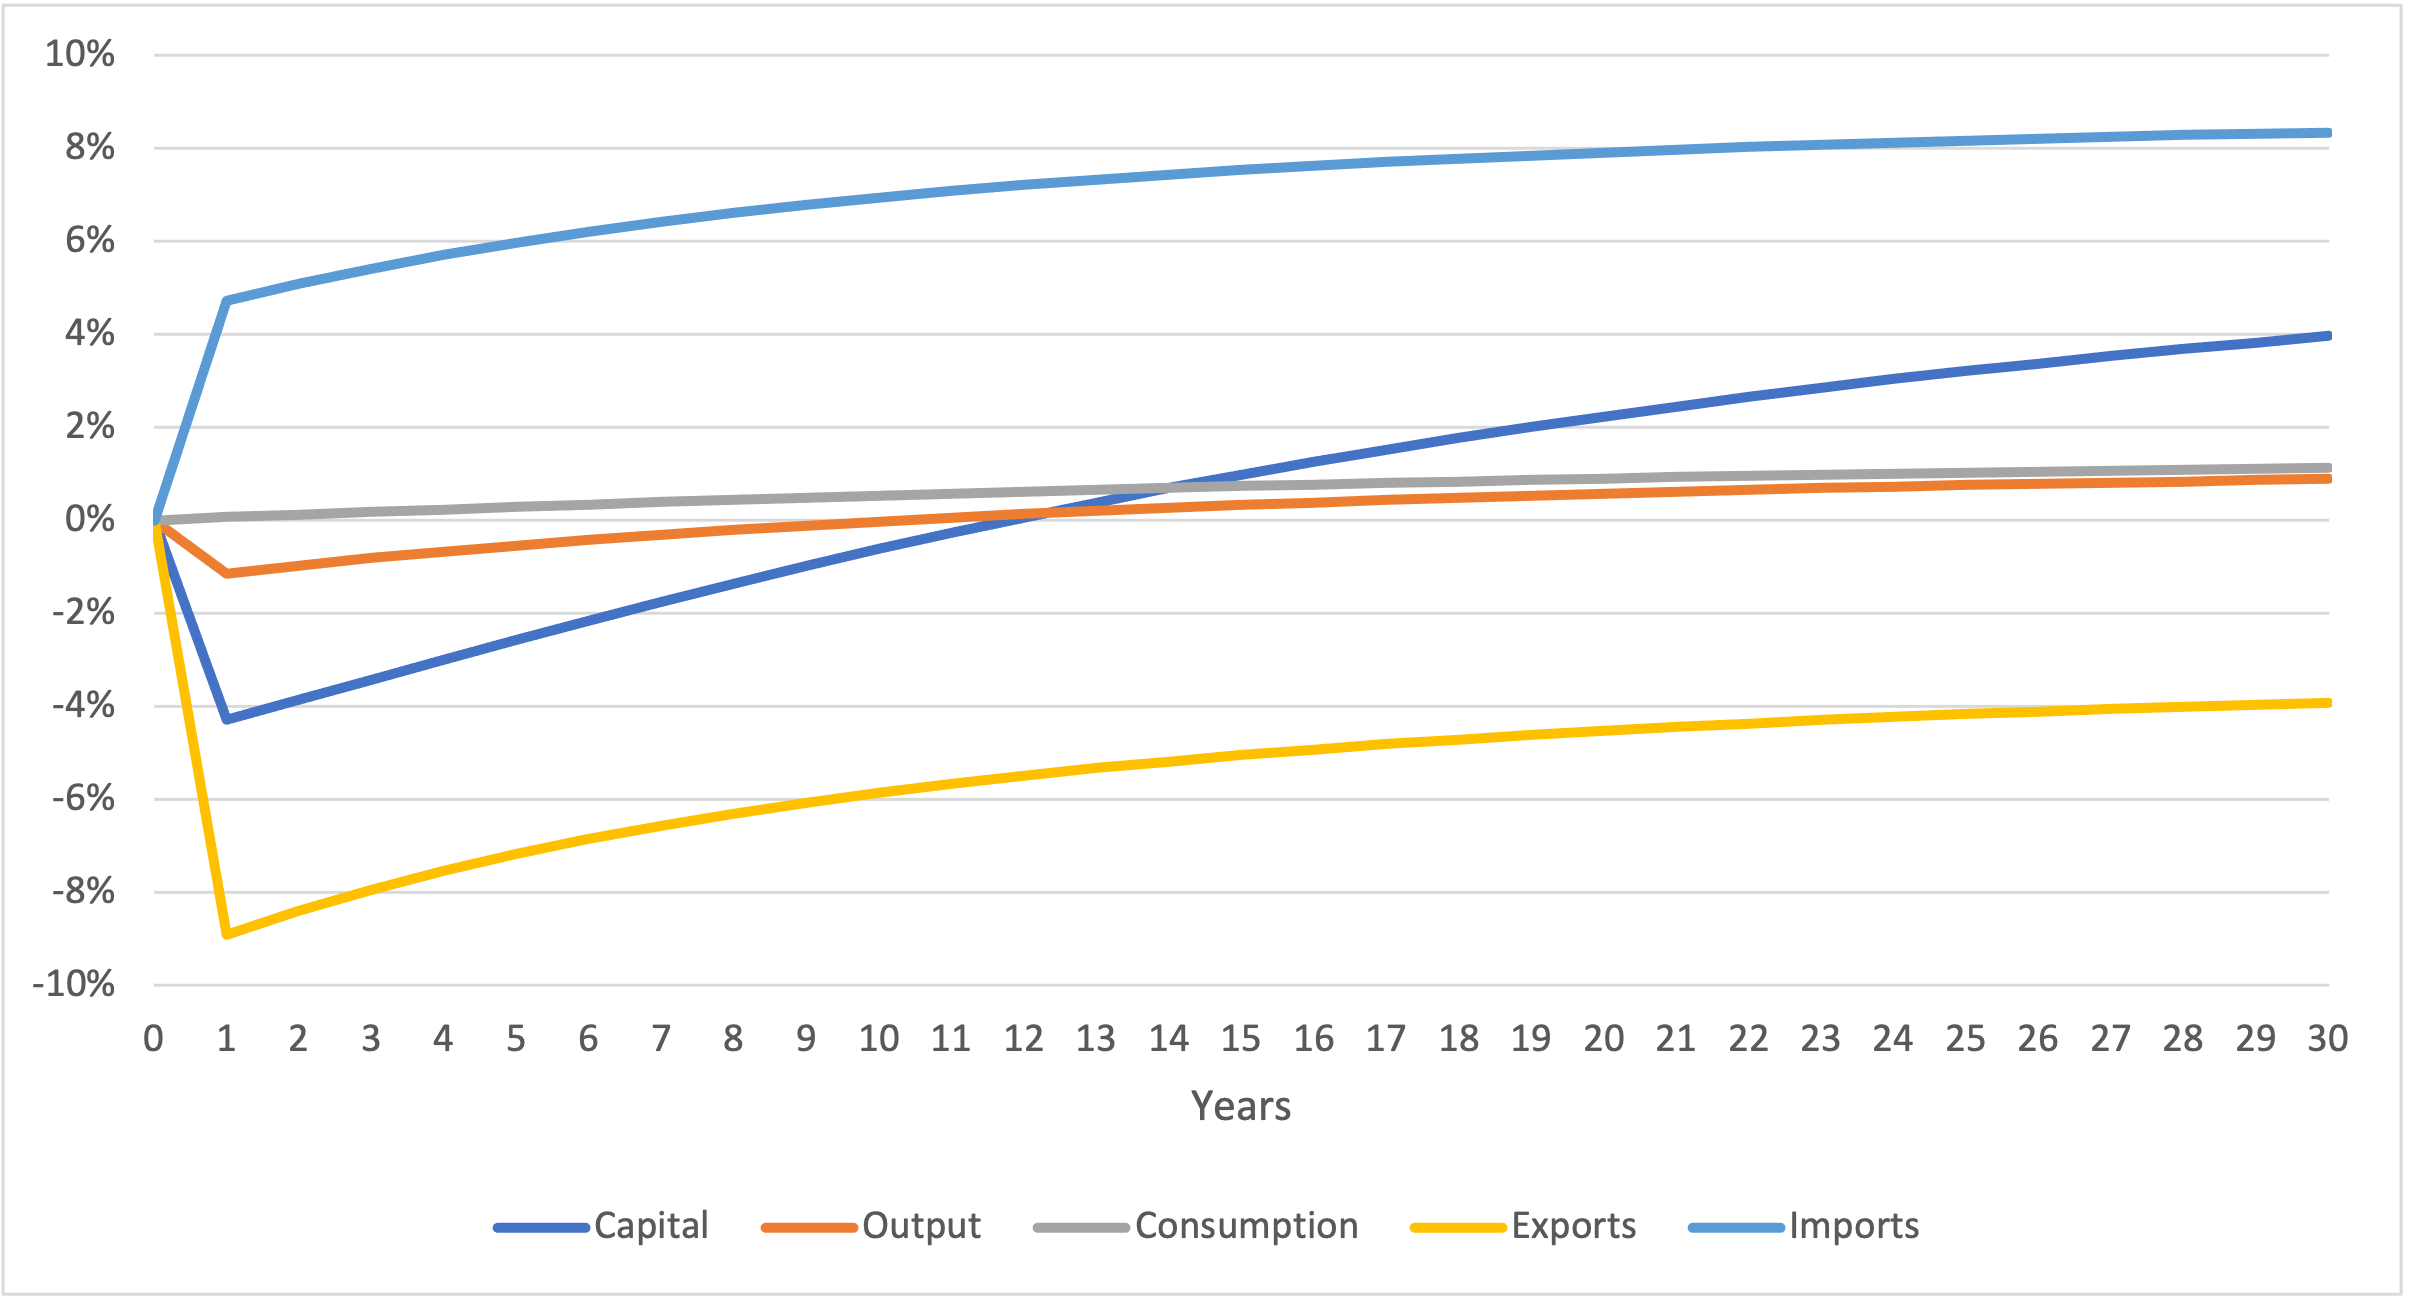
\includegraphics[width=0.98\textwidth]{_tex/agg-change.png}
\vskip5pt
   \caption*{\footnotesize 
   
   }
  \end{figure} 
%\begin{table}[H]
%  \begin{tabular}
%
%  \end{tabular}
%\end{table}


\begin{figure}[H]
  \caption{Agriculture: percentage change relative to status quo
 over time in years
  \label{fig-agg-change}}
 
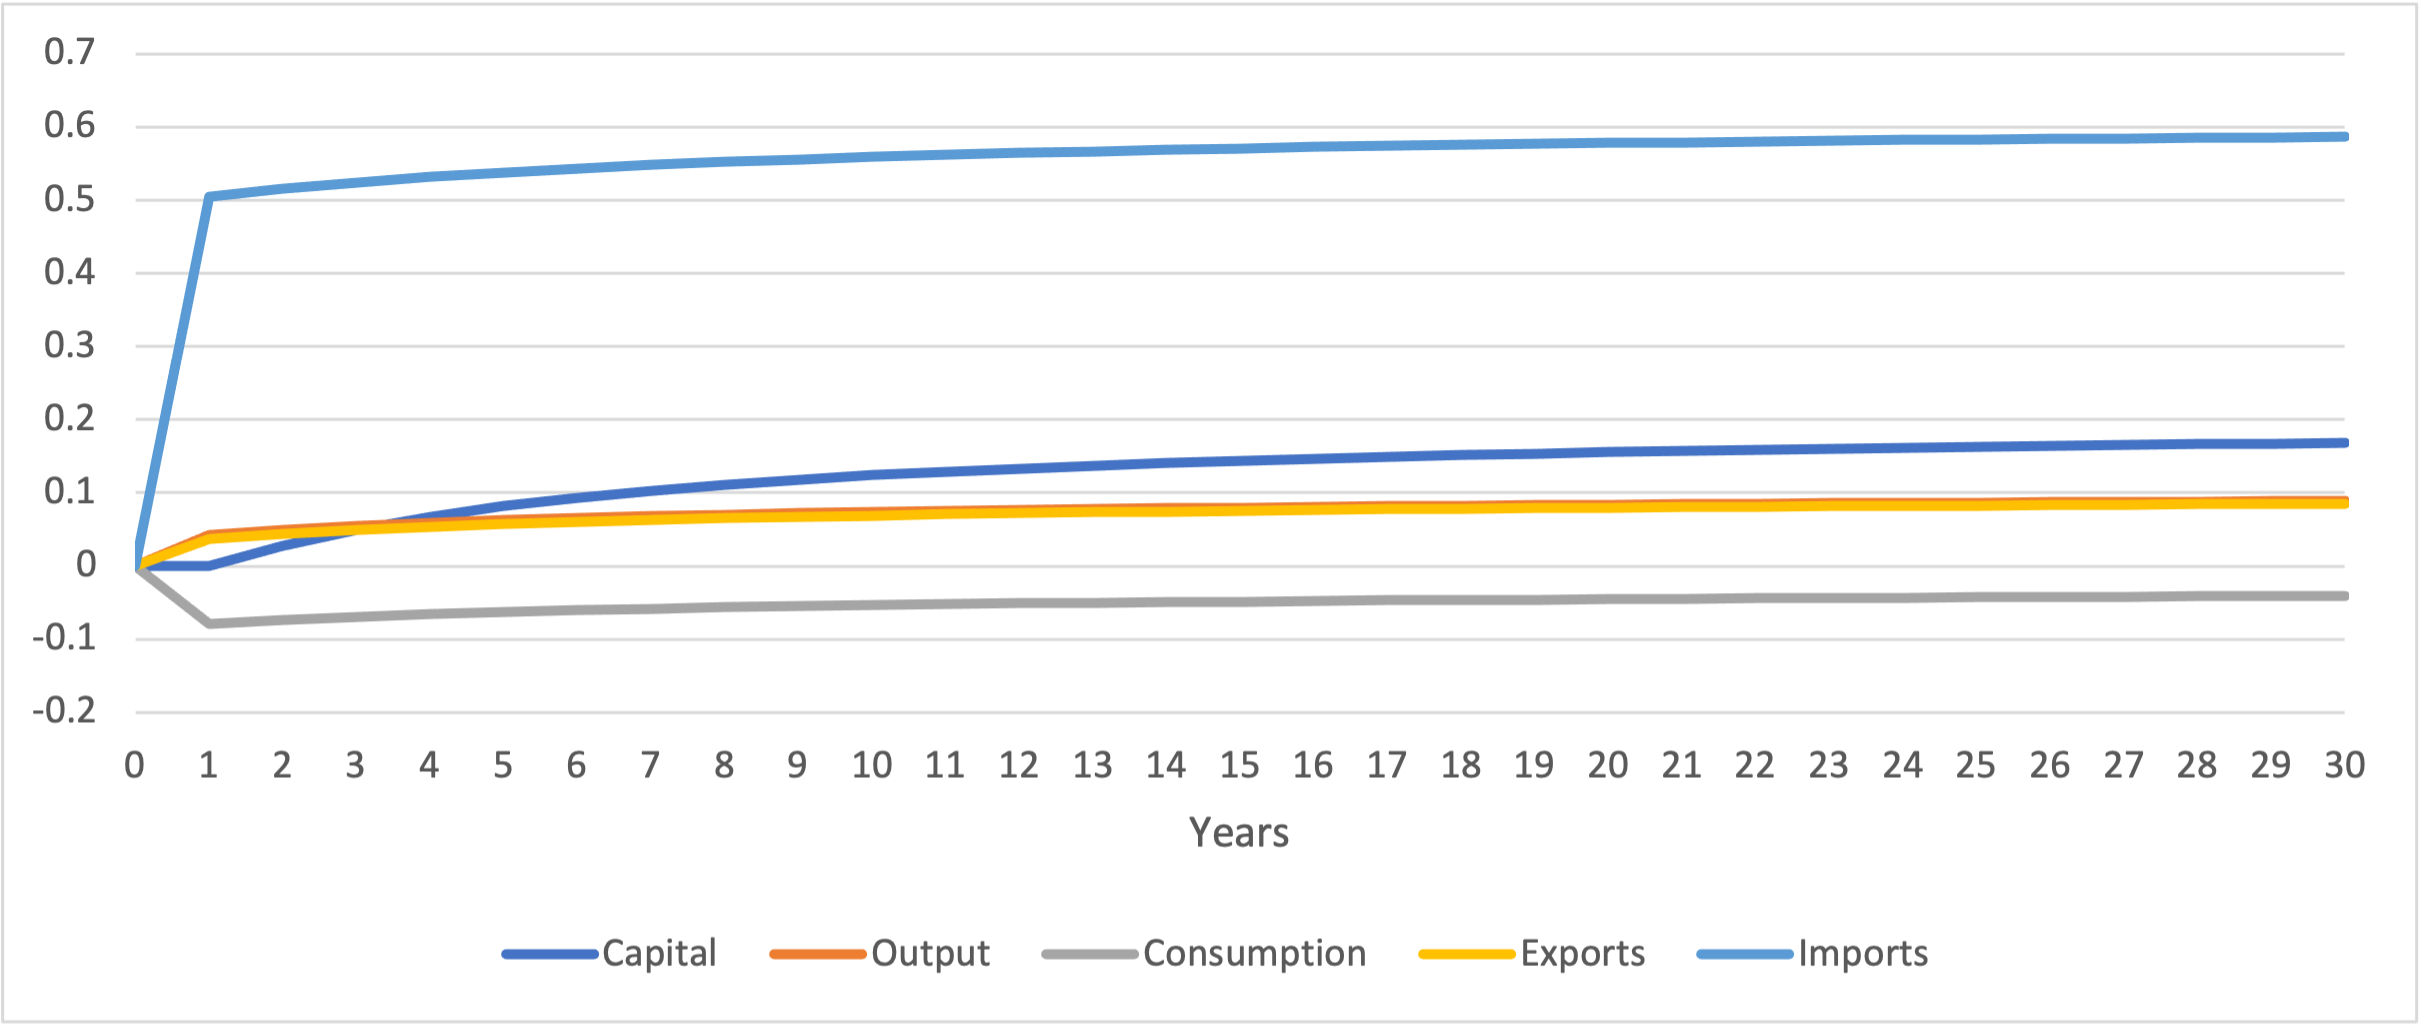
\includegraphics[width=0.98\textwidth]{_tex/A-change.png}
\vskip5pt
   \caption*{\footnotesize 
   
   }
  \end{figure} 


\begin{figure}[H]
  \caption{Mining: percentage change relative to status quo
 over time in years
  \label{fig-agg-change}}
 
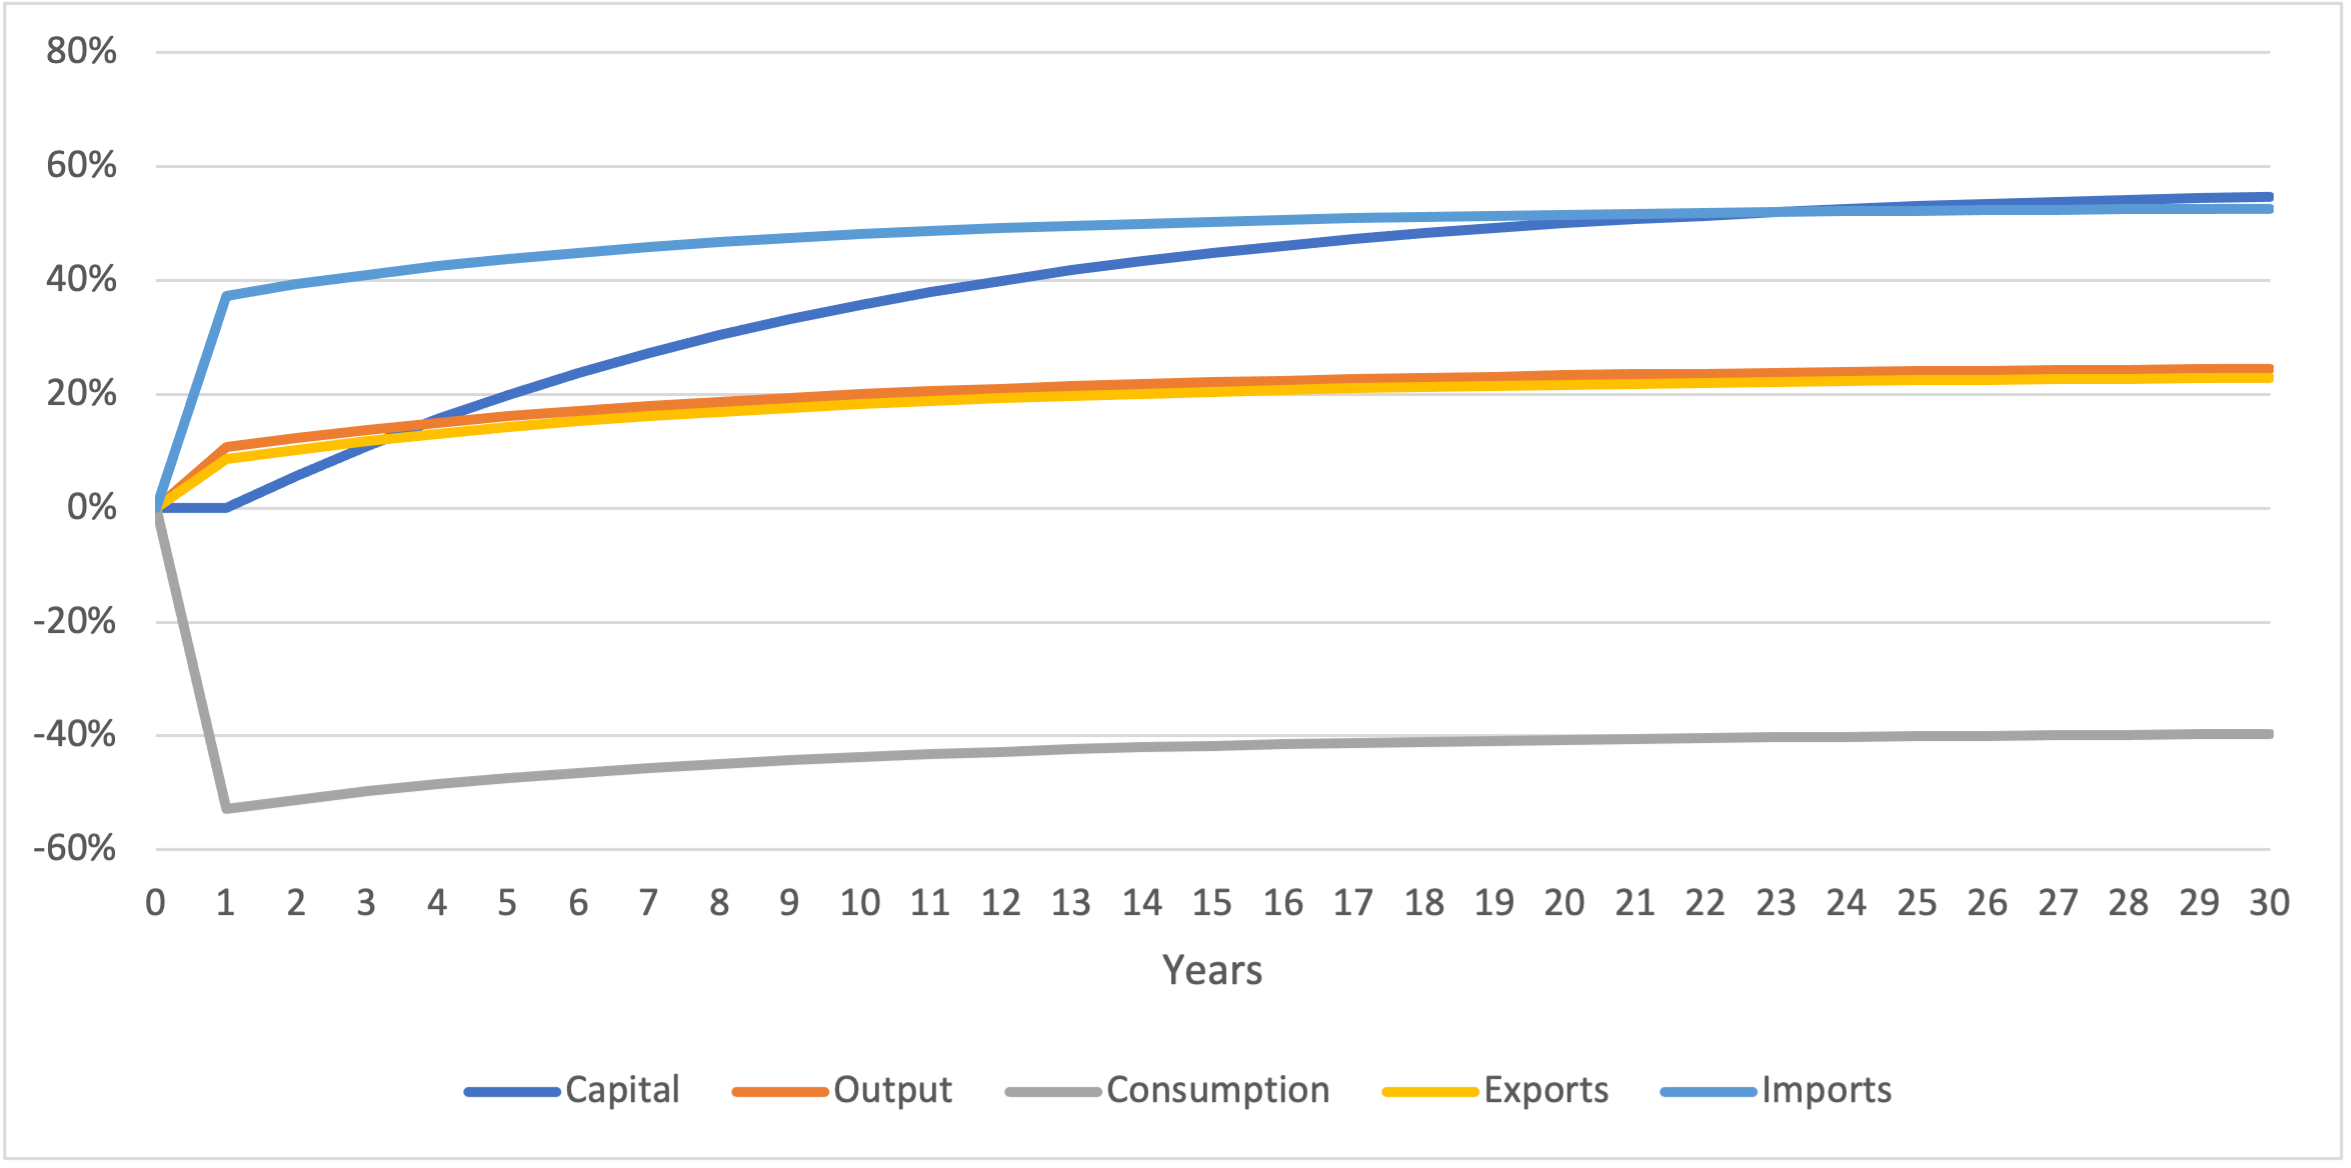
\includegraphics[width=0.98\textwidth]{_tex/B-change.png} \vskip5pt
\caption*{\footnotesize Note that although the change in consumption of mining
is large, it is only  a very small part of overall consumption } \end{figure} 

\begin{figure}[H]
  \caption{Manufacturing: percentage change relative to status quo
 over time in years
  \label{fig-agg-change}}
 
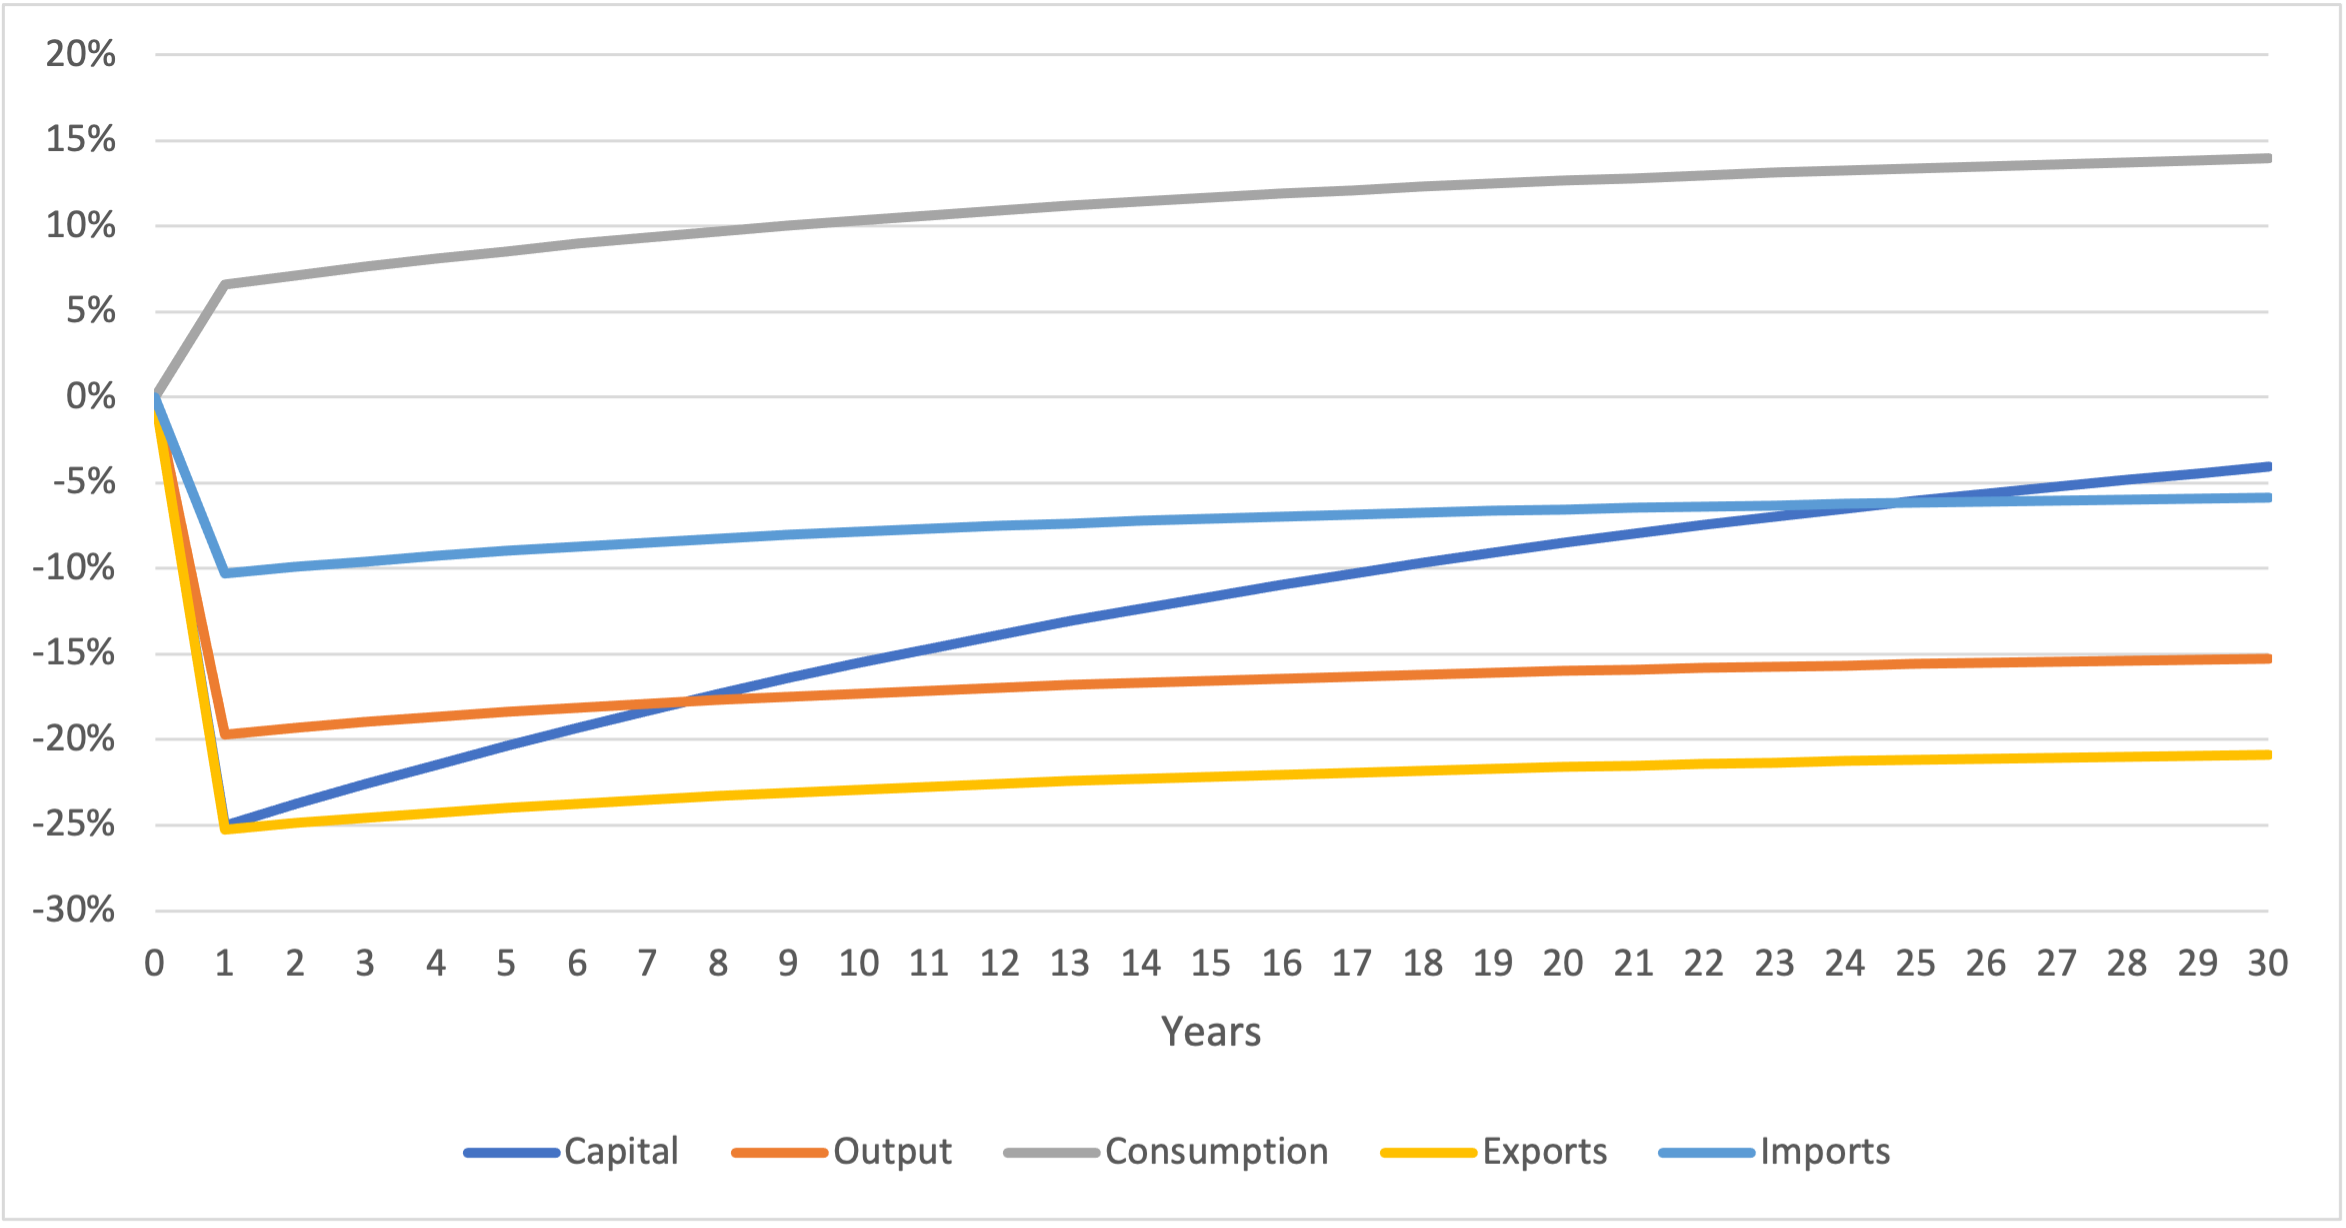
\includegraphics[width=0.98\textwidth]{_tex/C-change.png}
\vskip5pt
   \caption*{\footnotesize 
   
   }
  \end{figure} 

\begin{figure}[H]
  \caption{Utilities: percentage change relative to status quo
 over time in years
  \label{fig-agg-change}}
 
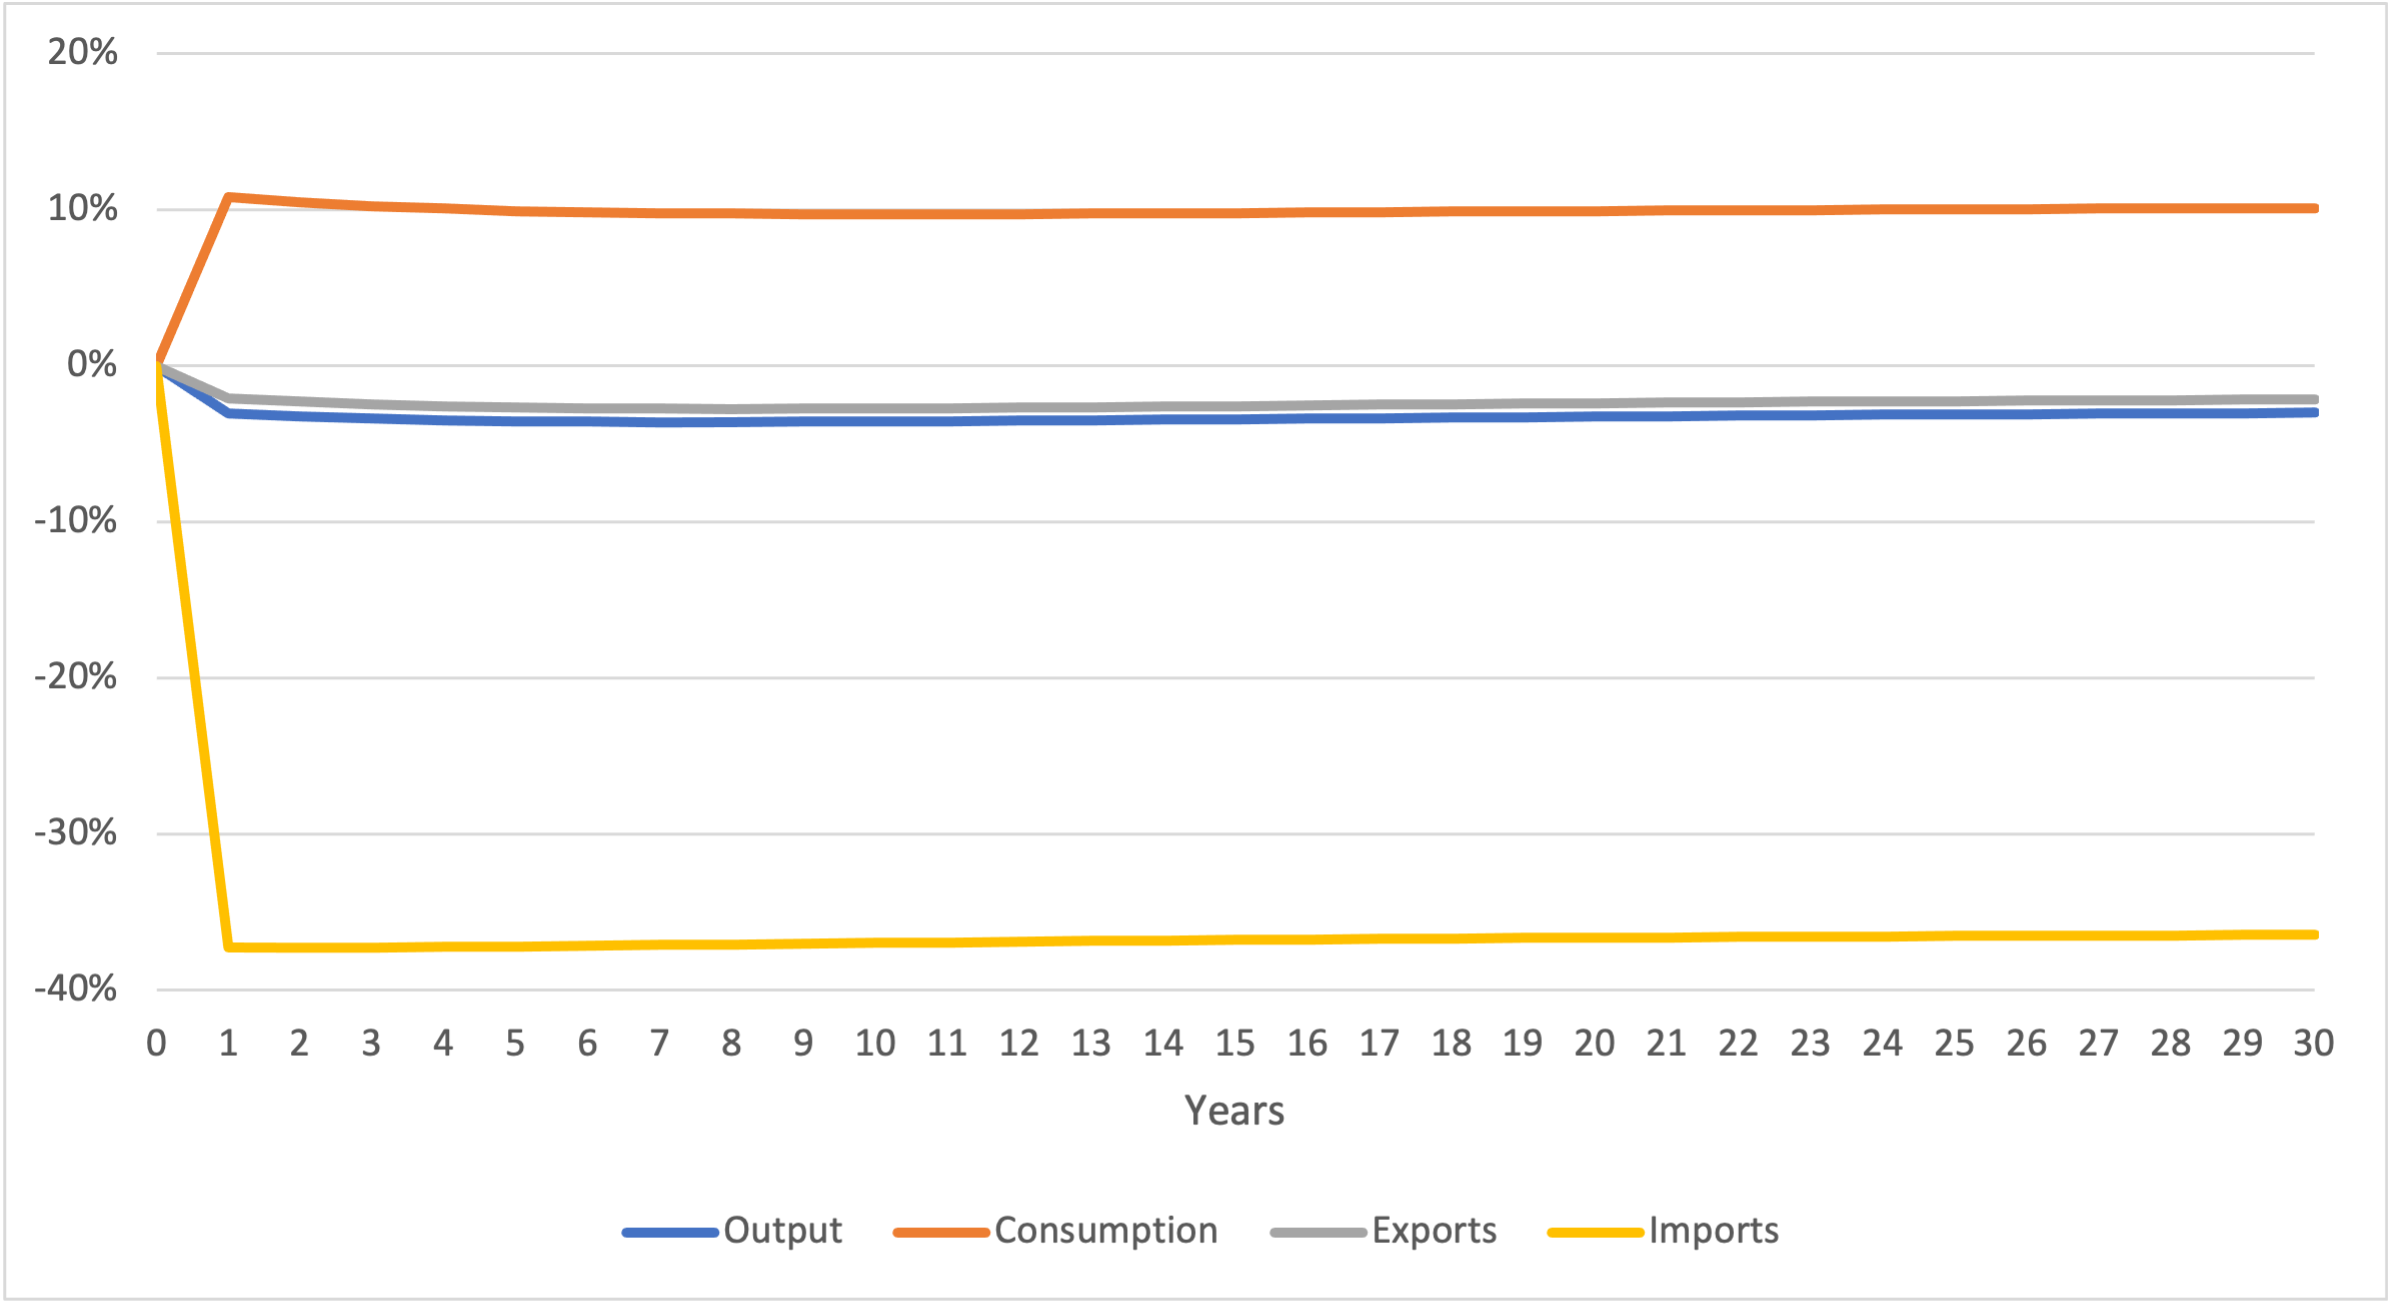
\includegraphics[width=0.98\textwidth]{_tex/D-change.png}
\vskip5pt
   \caption*{\footnotesize 
   
   }
  \end{figure} 

\subsection*{Future work} 

\paragraph{Robustness check} To ensure our conclusions are robust, we intend to
run a wider variety of shocks for a variety of parameterisations. This will
allow full features of the MAIWAR model to be brought to bear in analysing the
Greater Gladstone Economy (and other regions of interest in Queensland). In
particular, we will model different forms of adjustment paths, allow for
varying degrees of uncertainty and evaluate optimum policy options for the
Gladstone economy over time.

\paragraph{Allocating the smelter's land and capital to new production}
Following the closure of the Kurri-Kurri aluminium smelter in the Hunter
regions of New South Wales in October 2012, the process of decommissioning
began. Federal and state government approval to repurpose the site for a
gas-fired power station was finally given in December 2021: a full nine years
after the closure.  Our model is well-equipped to study the opportunity cost of
such delays.  In due course, we will look at future policy actions such as
putting the smelter capital such as land to different uses. BSL could for
instance be converted into a hydrogen processing plant or some other
green-energy facility. This could lead to a structural change and an increase
in the productivity of Manufacturing.  The model would be well-suited to
studying this with an emphasis on estimating the cost of delays and the
resulting unproductive capital. 



\begin{thebibliography}{1}

  \bibitem{aer} Australian Energy Regulator, Wholesale Markets Quarterly
    Report, Q2 2022, \url{https://www.aer.gov.au/system/files/Wholesale%20Markets%20Quarterly%20Q2%202022.pdf}

  \bibitem{Atalay} Atalay, Enghin. ``How important are sectoral shocks?,"
    American Economic Journal: Macroeconomics 9.4 (2017): 254-80.

\bibitem{Dann} Queensland Treasury Corporation (Peter Dann), “Boyne Island
  Smelter: Economic impact on the Gladstone Region and Queensland,” 2019

\bibitem{Brook}
Queensland Treasury Corporation (Peter Brook), ``Aluminium in QLD: Rio Tinto,” 2019
  
\bibitem{subsidies}
C. Hamilton and H. Turton, ``Subsidies to the Aluminium
Industry and Climate Change,'' The Australia Institute, 1999, https://www.tai.org.au/sites/default/files/WP21\_8.pdf

\bibitem{abs} Australian Bureau of Statistics (ABS), ``2016-2017 Table 5: Industry by
  Industry Flow Table (Direct Allocation of Imports),” released at 11.30am
  (Canberra time) 19 July 2019, https://www.abs.gov.au/AUSSTATS/abs@.nsf/DetailsPage/5209.0.55.0012016-17?OpenDocument

\bibitem{port}
 Port of Gladstone, ``Trade Statistics Data,''
 https://www.gpcl.com.au/trade-statistics, Retrieved  April 26 2020

\bibitem{RT}
  Rio Tinto, ``Annual Report: Production, Reserves and Operations,''
https://www.riotinto.com/invest/reports/annual-report, 2019, Retrieved on
27 April 2020

\bibitem{reg-prof}
  Queensland Government Statistician’s Office,
  ``Queensland Regional Profiles,”
https://statistics.qgso.qld.gov.au/qld-regional-profiles, Retrieved 26 April 2020 
 
\bibitem{id-comm}
  .idcommunity, “Regional resources,” 
  https:// economy.id.com.au/gladstone, Retrieved 27 April 2020

\bibitem{glad-prospectus}
  Gladstone Regional Council, ``Investment Prospectus'', Retrieved 25 September
    2022,
    \url{https://www.gladstone.qld.gov.au/downloads/file/3466/gladstone-region-investment-prospectus}

  \bibitem{manu-lab-share}
B. Berger and G. Wolff, “The global decline in the labour income share: is
capital the answer to Gernmany’s current account surplus?,” Policy Contribution,
Issue 12, April 2017

\bibitem{GPS-2029} Energy Matters, “Gladstone Power Station: We will operate
  beyond 2029,”
  https://www.energymatters.com.au/renewable-news/gladstone-power-station-remain-open-2029/,
  8 August 2018

\bibitem{AEMO} Australian Energy Market Operator, “2022 Integrated System
  Plan,”
    \url{https://aemo.com.au/-/media/files/major-publications/isp/2022/2022
    -documents/2022-integrated-system-plan-isp.pdf?la=en}

\bibitem{bat} G. Cusano, M. R. Gonzalo, F. Farrell, R. Remus, S. Roudier, L.
  Delgado Sancho,   “Best Available Techniques (BAT) Reference Document for the
    Non-Ferrous Metals Industries,” EUR 28648, doi:10.2760/8224, 2017

\bibitem{CSE}  
  CS Energy, ``Statement of Corporate intent," 2015/2016

\bibitem{GN-Aluminium-smelters}
  Gagne, R. , Nappi, C.  ``The cost and technological structure of aluminium
    smelters worldwide,'' Journal of Applied Econometrics, 2000, 15.4, Wiley,
    https://www.jstor.org/stable/2678590

%G. Eason, B. Noble, and I. N. Sneddon, ``,'' Phil. Trans. Roy. Soc. London,
%vol. A247, pp. 529--551, April 1955.

  

\end{thebibliography}

\end{document}



%%% Local Variables:
%%% mode: latex
%%% TeX-master: t
%%% End:

